\documentclass{protokoll_en}
\newcommand{\assistent}{M. Gr�ner}
\newcommand{\versuch}{Positron Lifetime in Metals and Insulators}
\newcommand{\nummer}{A246}

\newcommand{\Isotop}[2]{\ensuremath{^{#2}\mathrm{#1}}\xspace}
\newcommand{\vr}[2]{\ensuremath{\left(\begin{array}{c}#1\\#2\end{array}\right)}}
\newcommand{\Na}{\Isotop{Na}{22}}
\newcommand{\Ne}{\Isotop{Ne}{22}}

\begin{document}

\section{Preface}

\section{Theoretical Background}

\subsubsection{Natrium}
\label{cha:na}
To measure the lifetime of positron we need signals which start and stop the measurement. In the present experimental configuration \Na decays with an half-life of $\unit[2.6]{a}$ and a probability of $\unit[99]{\%}$ in the excited $2+$-state of \Ne via emitting a positron.
\begin{align*}
  \Na \rightarrow \Ne + e^+ + \nu_e
\end{align*}
We then use the detection of the $\unit[1245]{keV}$ line of excited \Ne into its groundstate as a starting signal (see also figure \ref{fig:natrium}). That is appropriate, because the excited \Ne state has a very short lifetime (approximately $\unit[10]{ps}$, while we expect a positron-lifetime of some nanoseconds). So one can argue that the moment of emission of the photon is indeed also the moment of the positron-creation.
\begin{figure}[H]
  \centering
  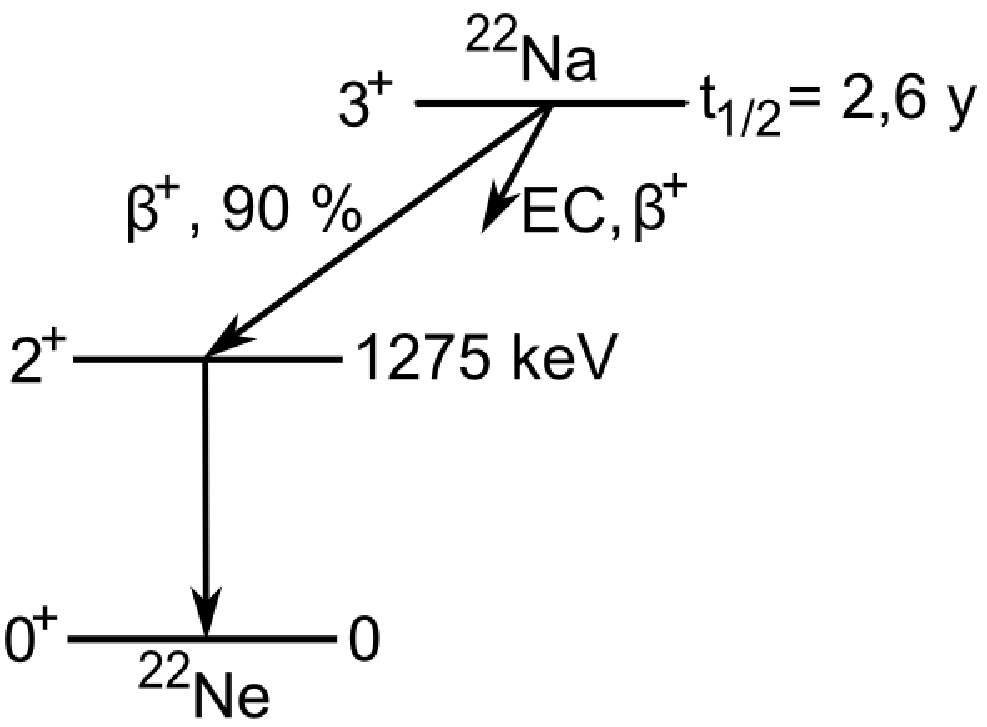
\includegraphics[width=0.5\textwidth]{graphics/natrium}
  \caption{Zerfallsschema von \Na~\cite{skript}}
  \label{fig:natrium}
\end{figure}
If a positron anihilates, two $\unit[511]{keV}$-photons are created. The detection of one of these stops the measurement.

\section{Experimentation and Analysis}


\section{Abstract}

\begin{appendix}

\section{Tables}

\Literatur{quellen}

\end{appendix}
\end{document}


